%!TEX root = paper.tex

% Brought from introduction
%NYC.gov \cite{nycgov} reports statistics and datasets for a range of domains such as emergency incidents, non-emergency events, crimes, offenses and more. NYC Open Data portal and the Office of Emergency Management (OEM) provide the Emergency Response Incidents dataset, which is publicly available at \cite{nycopendata} and is updated daily.

We use the emergency response incidents data from NYC Open Data provided by the Office of Emergency Management \cite{nycopendata}. We use around 8 years of data starting May 2011 to December 2019. The dataset consists of 13 incident types with 7 attributes each. We use three attributes from the dataset --- Incident type, Creation date, and Close date. In this study, we focus on three of the most important and frequent emergency types --- \textit{Fire}, \textit{Law}, and \textit{Structural}. We calculate the {\it resolution time} for each incident by subtracting the creation date from the close date and converting it to minutes. %and Utility. 
Figure \ref{fig:trend} shows the resolution times for these incidents. We observe that the time required to resolve events related to \textit{Law} is the least followed by %utility, 
\textit{Fire} and \textit{Structural}, respectively. We also observe from Figure \ref{fig:trend} that there is significant variation in resolution time for events belonging to the same incident type.

%In this section, we explain with more detail the reasoning behind our preprocessing criteria and show how some statistics varies according to this, Table \ref{table:stats} shows the response time statistics (mean, standard deviation) for the four incident types before and after the preprocessing steps. 

{Additionally, we observe from the data that each of these three incident types have multiple subtypes, which we extract from the type description.  \textit{Fire}, \textit{Law}, and \textit{Structural} have 52, 29, and 73  subtypes, respectively.  Figure \ref{fig:subtype} shows the  incident subtypes that contribute the most events for each of the most general incident types. We observe that \textit{2nd alarm}, \textit{Suspicious Package (denoted as Package)}, and \textit{Collapse} %and \textit{Water Main} 
are the subtypes that account for the highest number of events in \textit{Fire}, \textit{Law}, and \textit{Structural}%and Utility 
, respectively.





\subsection{Preprocessing}
\label{Data:Preprocessing}

As is the case with most data-driven solutions to real-world problems, the first step involves pre-processing the data to identify missing values and outliers.  We observe that the dataset contains non-trivial number of missing values for events. A missing value is encountered when an event does not have  a valid close date. In the entire dataset, we observe that  \textit{Fire}, \textit{Law}, and  \textit{Structural} have 32\%, 12\%, and 23\%  missing values, respectively.  For each incident type, we replace these missing points by sampling from the actual distribution of the remaining points. To determine the actual distribution for each incident type, we fit the data to more than 80 different distributions. We perform  the Kolmogorov-Smirnov  goodness of fit test (KS test) and use the \textit{p-value} of the KS test to pick the best distribution for the dataset under consideration. 


%We select the distribution with the maximum $p\_value$. If we happen to get some negative values or outliers again, we replace them with zero and quantile 90 of the incident type respectively. We support and explain with more details all these preprocessing decisions in section \ref{Data:Discussion}.

%and utility has 31\% 


We also observe that the dataset contains some outliers---values that are significantly different from the rest of the data points.  By studying the values, we believe that such values might be the result of manually closing some unfinished entries at a later date. For example, we observe some extreme outliers in the dataset (greater than 100,000 minutes). We identify outliers as those points whose resolution time is greater than the quantile 90 of that incident type. For  \textit{Fire}, \textit{Law}, and  \textit{Structural}, we observe that there are 7\%, 9\%, and 8\% outliers, respectively.  Figure \ref{fig:before_after} shows the distribution of  the three different incident types before and after preprocessing.  We observe from the figure that the raw dataset has a large number of outliers.  We once again replace these outliers by sampling from the  distribution of the valid data points. In comparison  to Figure \ref{fig:beforeprocess}, we observe that Figure \ref{fig:afterprocess} presents a significantly refined distribution.


\begin{figure}[!ht]
    \centering
  \subfloat[Before preprocessing]{%
       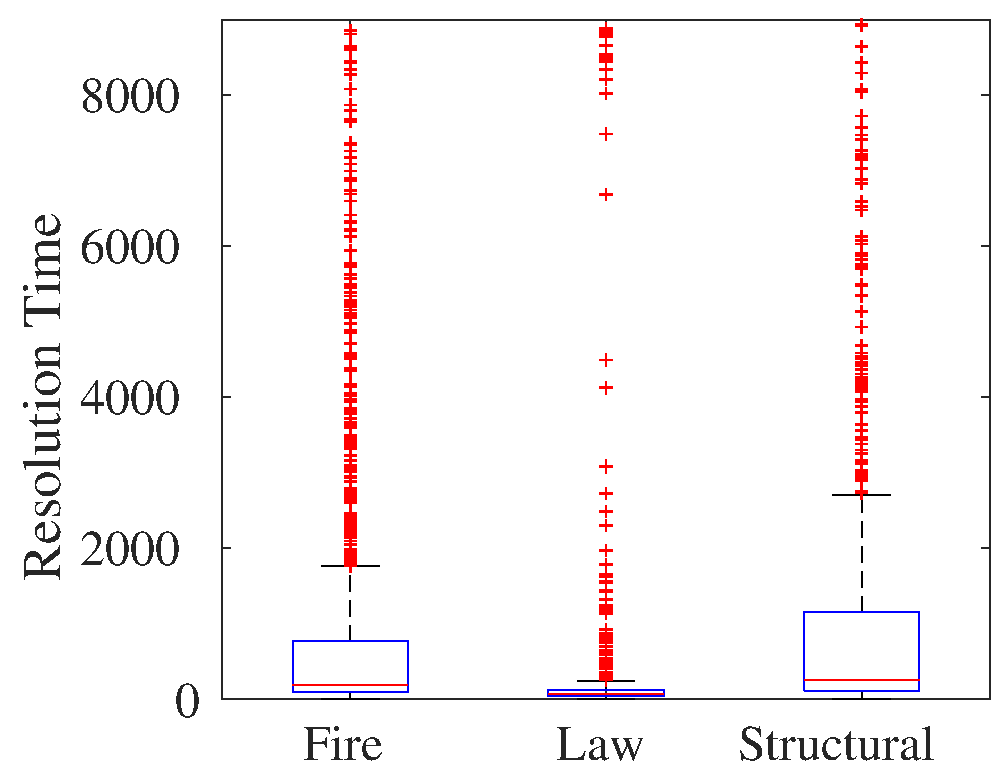
\includegraphics[scale=0.25]{Figures/Data/Boxplot/All_Incidents_before}
       \label{fig:beforeprocess}}
%  \vspace{1mm}
  \subfloat[After preprocessing]{
       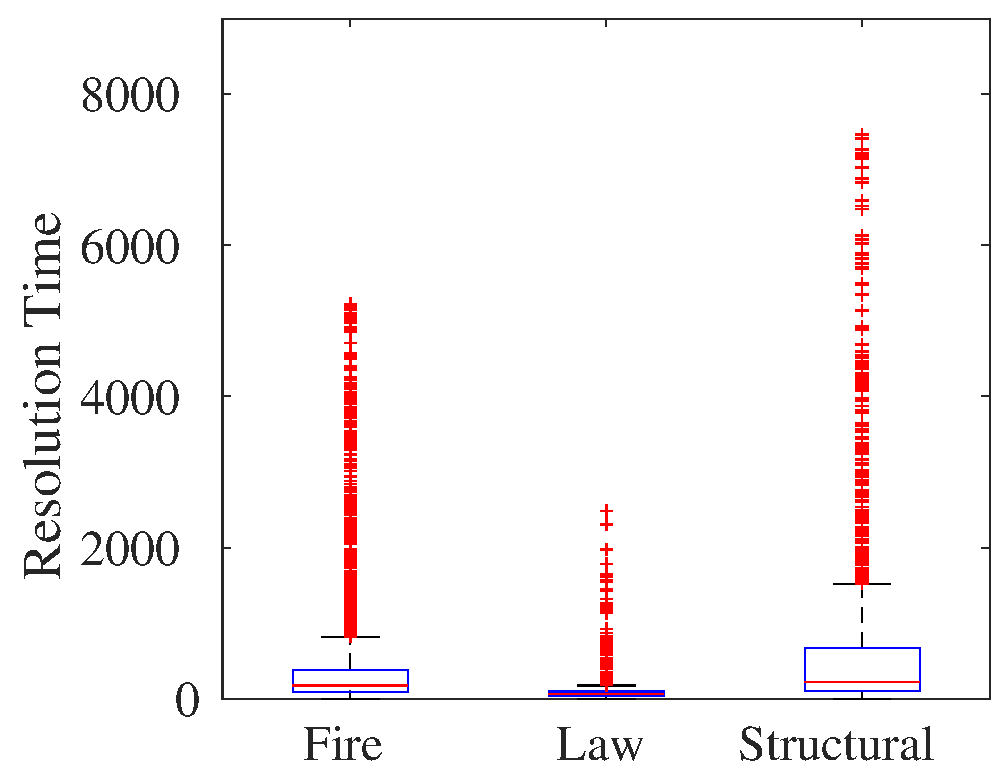
\includegraphics[scale=0.25]{Figures/Data/Boxplot/All_Incidents_after}
       \label{fig:afterprocess}}
	\caption{Datasets before and after preprocessing}
  \label{fig:before_after} 
  \vspace{-1mm}
\end{figure}


We observe some other interesting issues in the dataset. We observe that for {\it Fire} and {\it Structural} most of outliers are located in the first  few years of the dataset. In comparison, most of the missing points are located during the last few years.  Additionally, for {\it Fire} and {\it Structural} we observe larger resolution times during the initial years than the last few years. However, the opposite is true for \textit{Law},  where the resolution times during the initial years is lower than the resolution times in the later years. 


%We use two approaches to perform this replacement --- 1) Sample randomly from the valid points of the training set, and 2) Fit a distribution to each incident type and sample continuous values from these distributions using training set. 


 %\blue{As both these approaches show similar results, in the rest of the paper, we only report results using the second replacement approach.}





%On the other hand, before preprocessing, the values of outliers are very large although , for visualization reasons.
%the input and prediction lengths $m$ and $k$. 








%We aim to design a model that is flexible enough to model any sequence of incidents time frame and can recognize patterns independent of the frame duration. For this time series problem, instances of consecutive fixed number of incidents belong to different time frames. 


%%%%%%%%%%%%%%%%%%% CONFIRM: table values PREV without outliers





%\begin{figure}[!ht]
%    \centering
%  \subfloat[Fire]{%
%       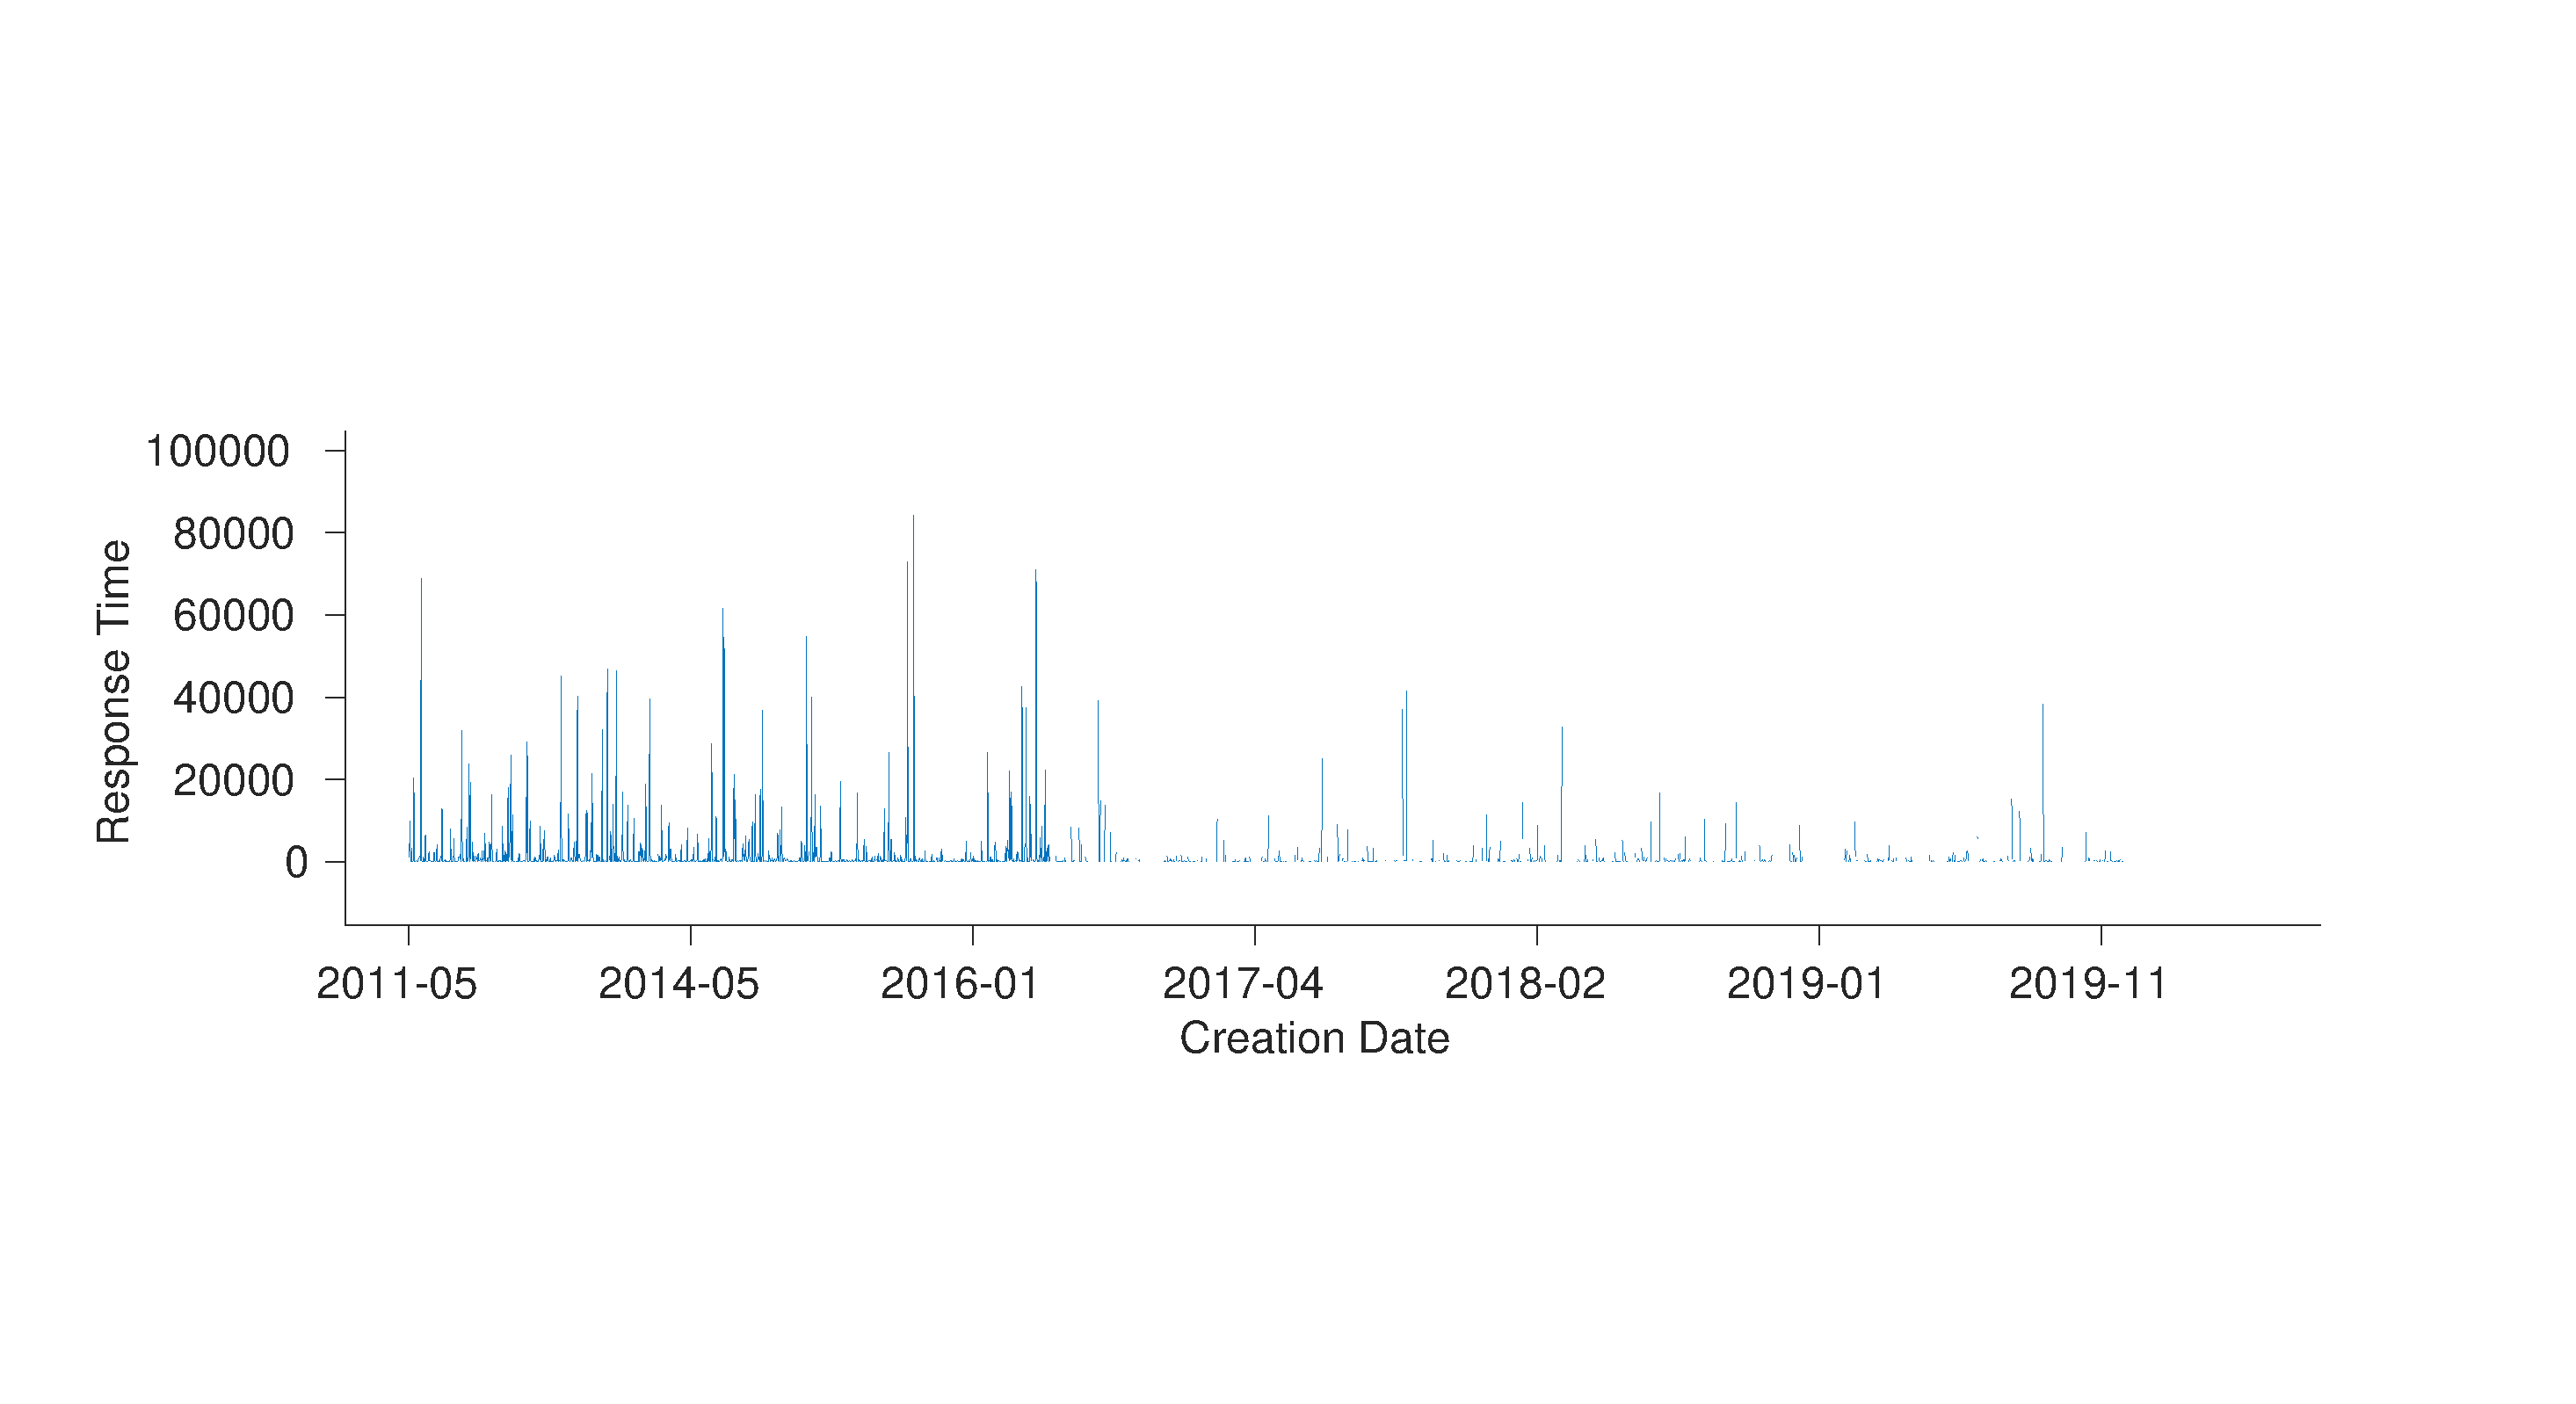
\includegraphics[trim=40 150 150 200,clip,width=1.0\linewidth]{Figures/replacementBinary/plotOutMissFire_mat}%[trim=130 250 150 250,clip,width=1.0\linewidth]{Figures/replacementBinary/plotOutMissFire_mat}
%       \label{4a}}
%  \vspace{1mm}
%  \subfloat[Law]{%
%       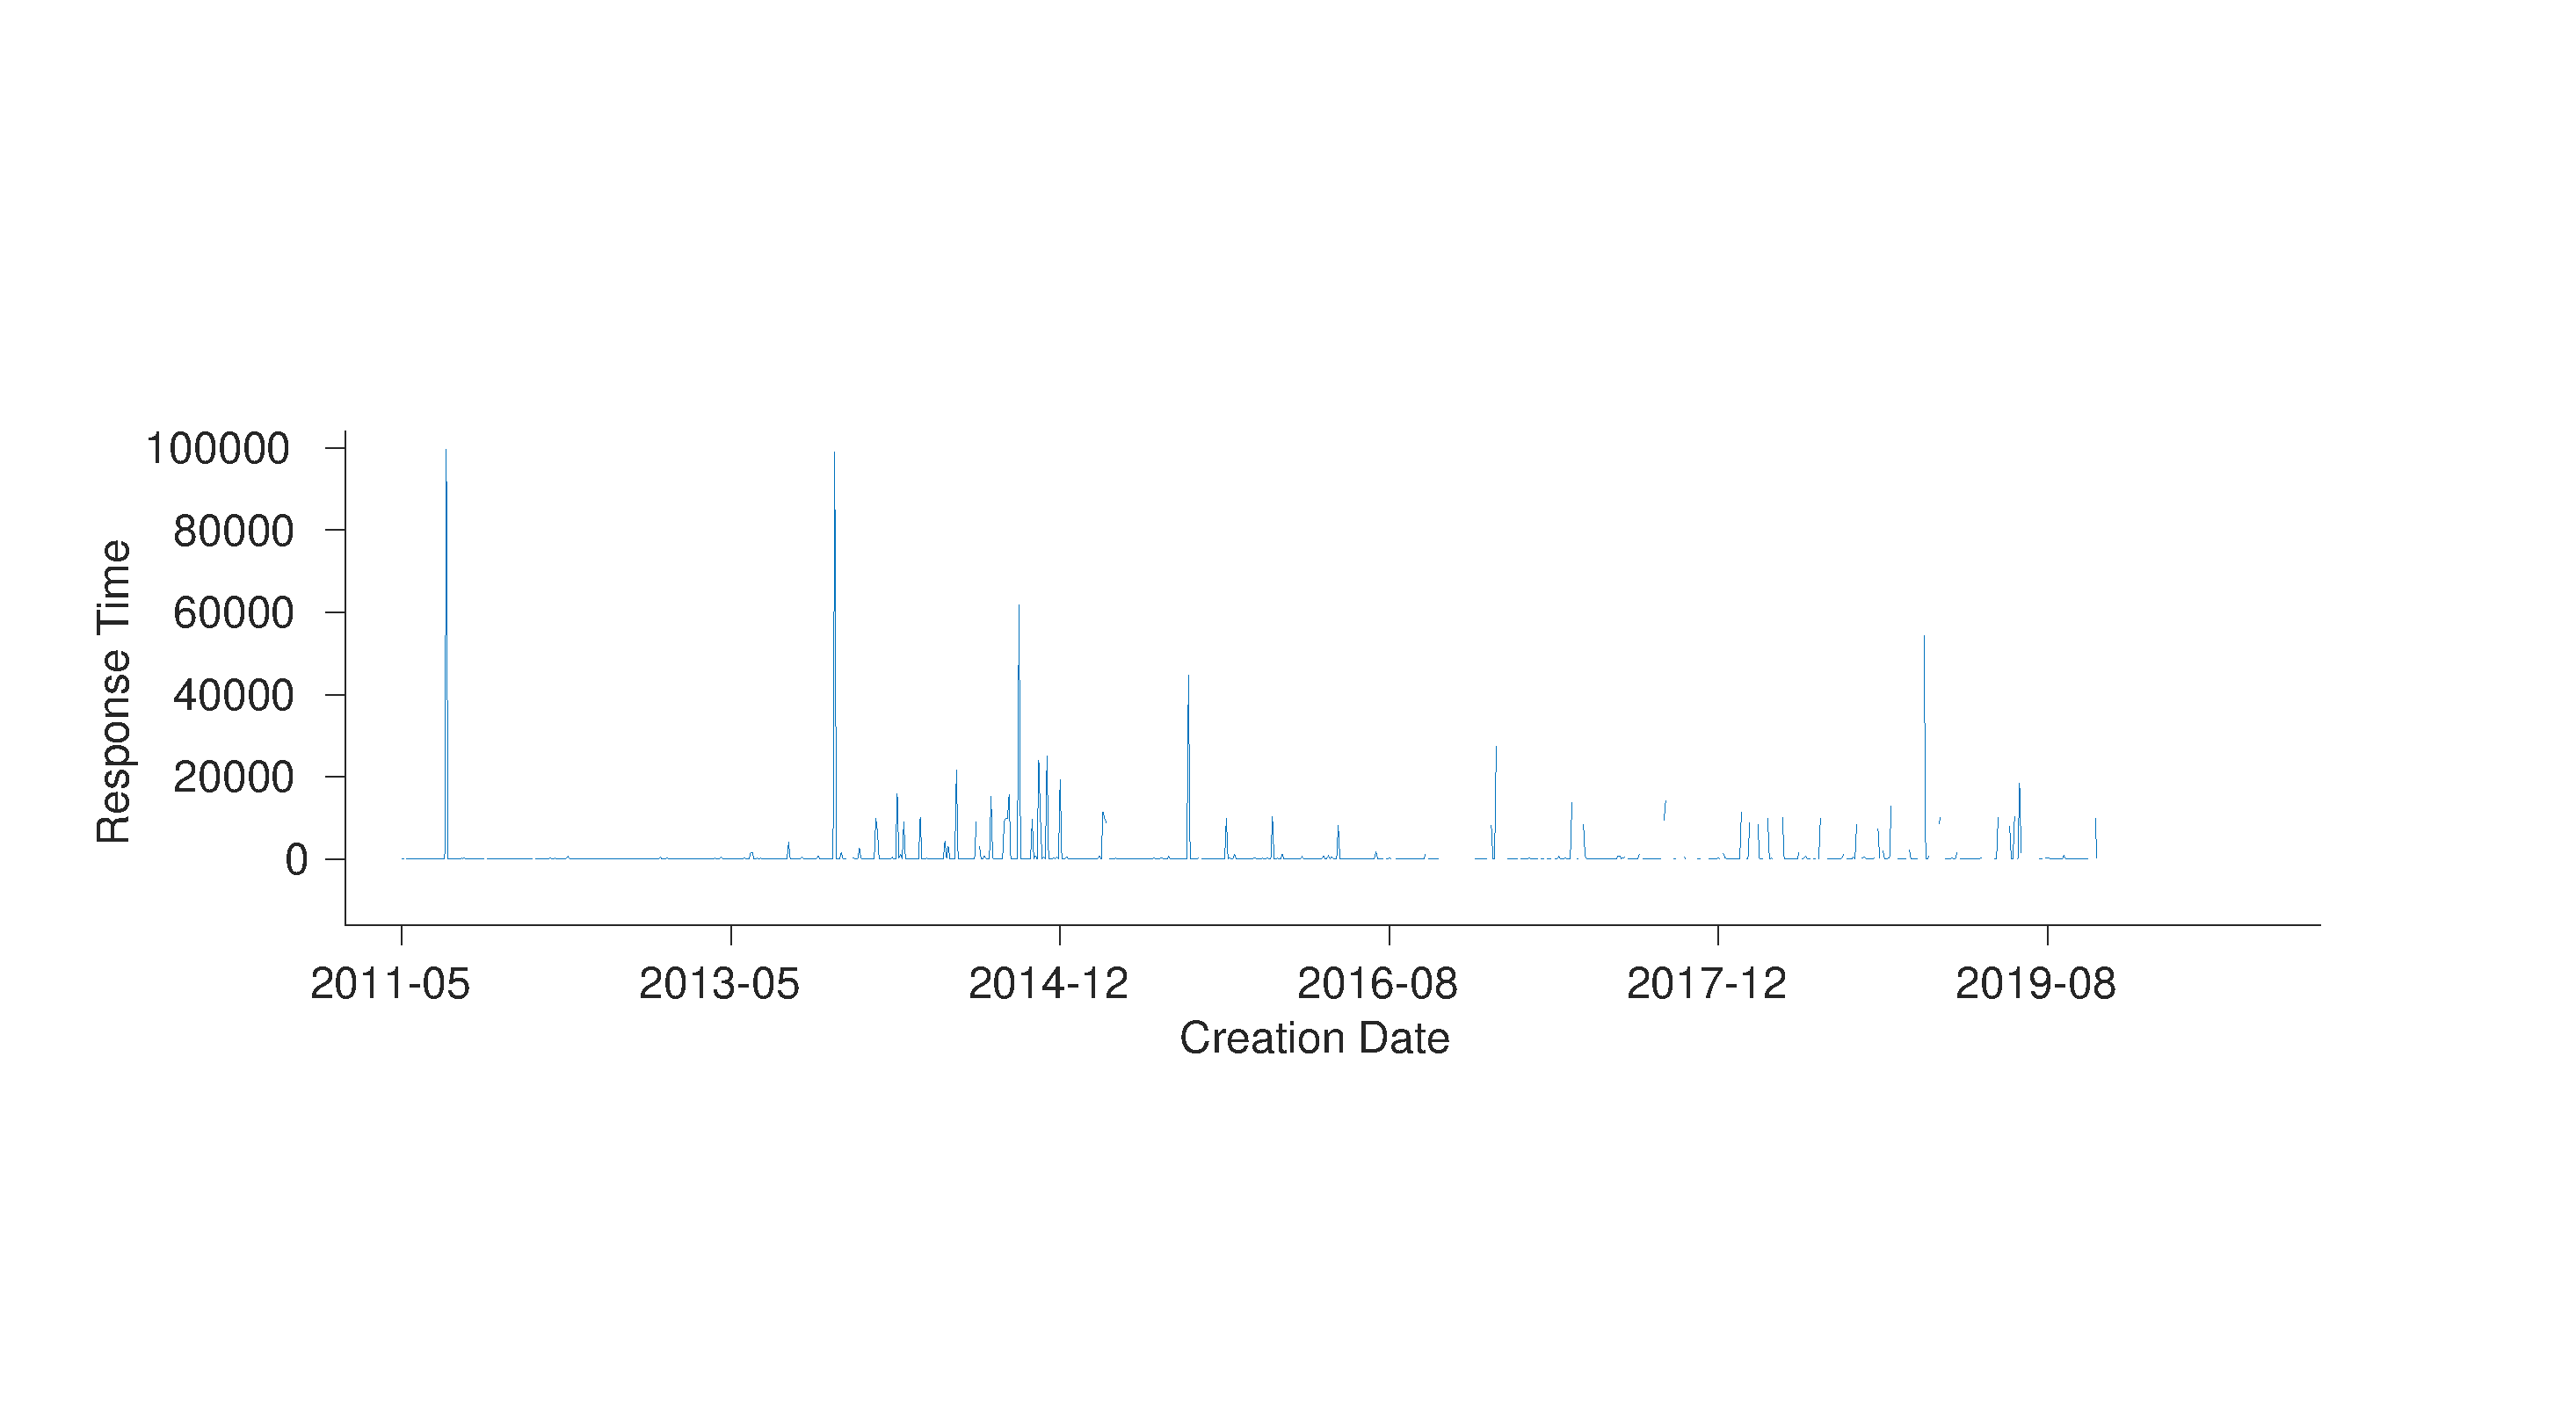
\includegraphics[trim=40 150 150 200,clip,width=1.0\linewidth]{Figures/replacementBinary/plotOutMissLaw_mat}
%       \label{4b}}
%  \vspace{1mm}
%  \subfloat[Structural]{%
%       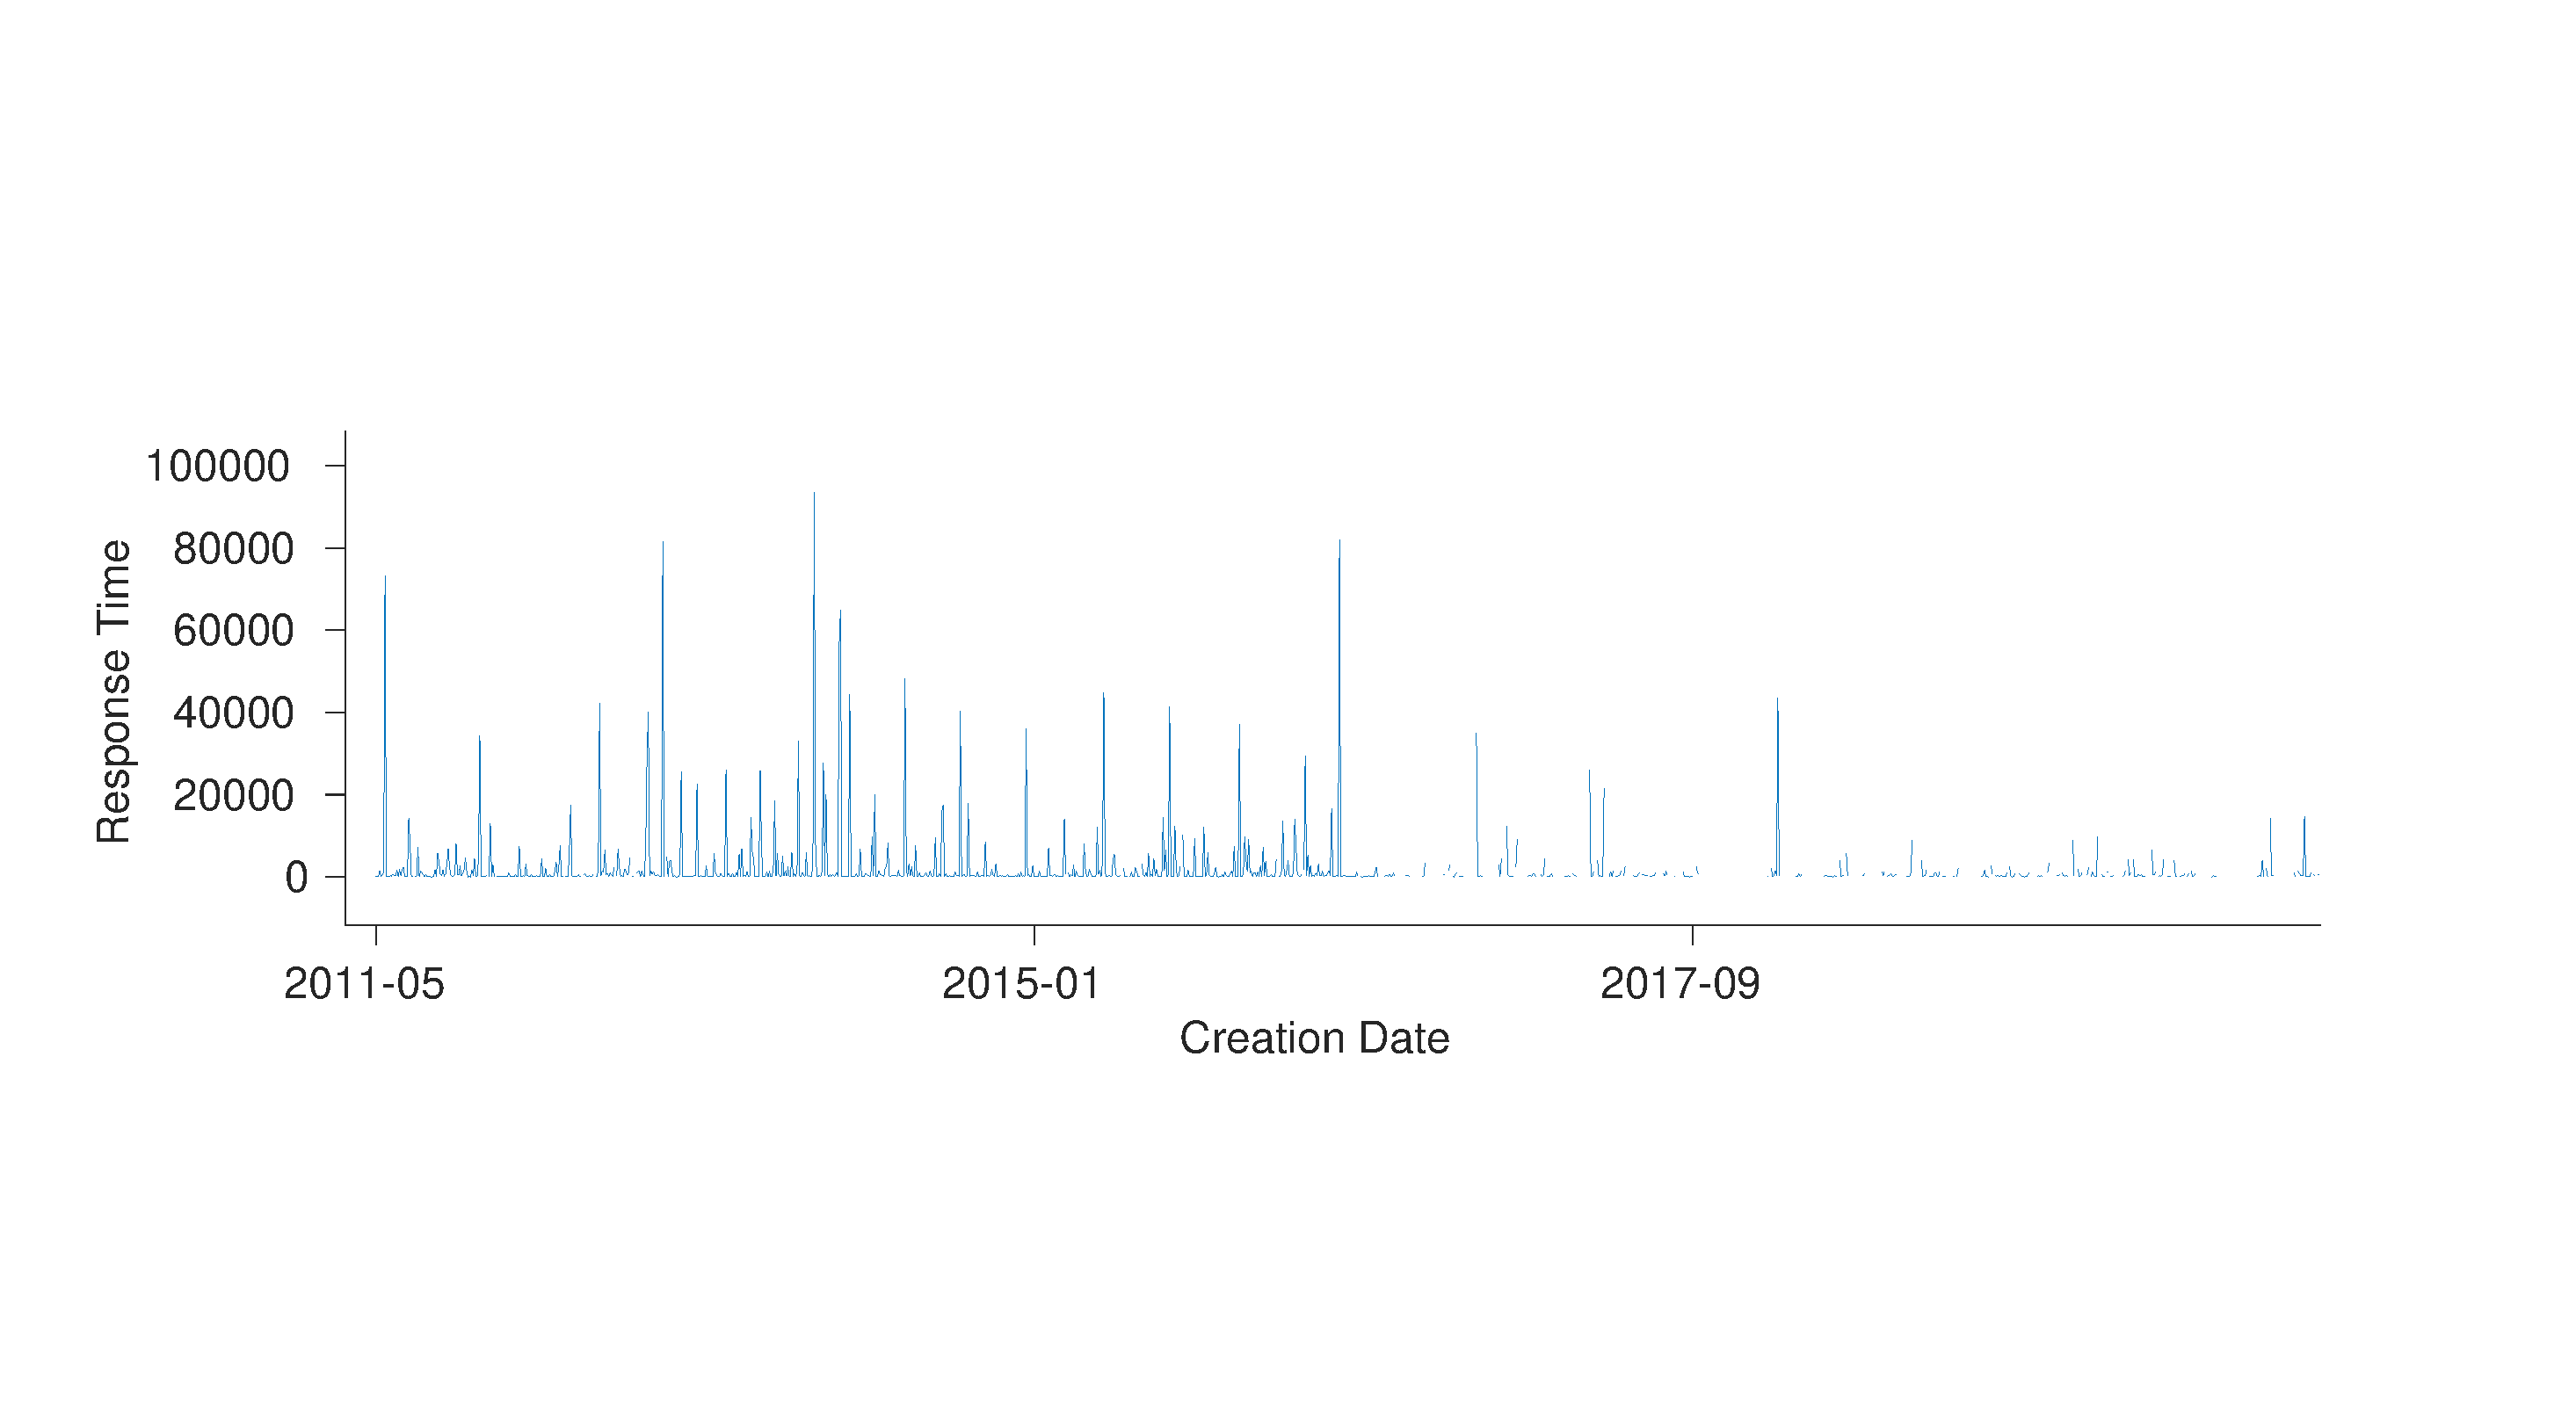
\includegraphics[trim=40 150 120 200,clip,width=1.0\linewidth]{Figures/replacementBinary/plotOutMissStructural_mat}
%       \label{4a}}
%  \vspace{1mm}
%  %\subfloat[Utility]{%
%  %     \includegraphics[scale=0.26]{Figures/replacementBinary/plotOutMissUtility.png}
%  %     \label{4b}}
%	\caption{Graphical location in time of outlier and missing values}
%  \label{fig:missingValues} 
%  \vspace{-1mm}
%\end{figure}




%The response time of an event is estimated by the difference between the close date and the creation date of it. Figure \ref{fig:subtype} shows the distribution of reponse time for some subtypes of the groups of events we choose for this work. Although the range of these distributions are wide, our model accomplishes to estimate a response time more accurate that the baselines we use. 
%Together with a model to determine when the next event would occur, this model can support assignment of resources and logistics decisions to improve response for future events.